%! TEX root = thesis.tex
% vim: ft=tex et sts=2 sw=2

\chapter{Comments and TODO}

\section{Comments on Paper 1}

\begin{enumerate}
  \item In the derivation for regular points, it's not readily clear that the matrix in the exponential would be positive definite.  But this is so since it's the Hessian of a function ($=U(q) + |\hat{\vartheta}(q) - \vartheta|^{2}$) which has a minimum at $q_{i}$.
\end{enumerate}

\section{Comments on Paper 2}

\begin{enumerate}

  \item What's the connection between the Faddeev--Popov method and the coarea formula?  See Zee's book on QFT.
  \item Language: point \emph{in} manifold or point \emph{on} manifold? N.B. a manifold is a set.
  \item I didn't use the constant-rank theorem since that'd require more explanation, e.g., there could be rows of the Jacobian that are \emph{not} independent if the requirement is only constant rank.  Perhaps we can add that preimage theorem, constant-rank theorem, etc., are variations of the implicit function theorem.
  \item I'm being purposefully sloppy in the definition of the tangent space.
    The vectors $\bm{v}$ should be picked from $T_{\bm{q}} \mathcal{Q}$ (in which case I'll need to define that first) and not $\mathbb{R}^n$.
    Here it's okay since $\mathcal{Q}$ is always considered as a submanifold of $\mathbb{R}^n$, which makes $T_{\bm{q}}\mathcal{Q} = \mathbb{R}^n$.
  \item What's the guarantee that a rank deficiency leads to a bifurcation?  Also, rank-deficiency singularities could be parameterization singularities.  I think CS singularities require rank deficiency, but rank deficiency doesn't always guarantee CS singularity.
  \item A zero mode is technically a motion on the tangent bundle $TM$ since you want $q \in \Omega$ and $v \in T_{q}\Omega$.
  \item Even though $q$ and $v$ belong to different spaces we are taking $q \to q + v$.  Although I'm confident that there's nothing wrong with this, I want to understand this better.  Goes back to CM where we take $q \approx q_0 + v t$.
  \item What's the connection between energy near a singularity and the ``affine energy'' in Lubensky et al.'s RPP review (Eq.~3.10)?
  \item Even though zero modes corresponding to flexes don't cost energy, we still have $x\trans\hess f_ix \neq 0$.  This is because flex is ``nonlinear''.  However, the partition function calculation is still fine because the projection operator will kill these nonzero terms.
  \item In our discussion, we have focused on self stress states of points that belong to the constraint manifold.
  However, we should note all points $q \notin \Omega$ for which $C(q)$ drops rank, also admit self stress states.
  Discuss issues, e.g., drop in rank doesn't guarantee singularity, etc.
  \item Can you call an ordinary function positive definite or positive semidefinite?
  \item If $A + B = C$, where $A, B, C$ are vector spaces, does one say that $A$ and $B$ spans $C$ or $A$ and $B$ generates $C$?  Or are both wrong?
  \item Plot $\beta F(\xi)$ instead of saying that you're plotting free-energy in units of $\beta^{-1}$.
  \item Histogram method for free energy is also called ``visited states method''.
  \item What's the guarantee that states of stress (and singularities) are gauge invariant w.r.t. the local body frame of the mechanism?
    Gauge invariance in the sense of Littlejohn's papers on few-body systems.
  \item Adjacency matrix = sign(compatibility matrix)?
  \item To write the partition function as the Laplace's transform of the density of states, shouldn't the energy function $U(\bm{q})$ foliate $\mathbb{R}^{n}$? Coarea formula.

  \item Out of plain buckling of thin plates, Foppel-von Karman limit, stresses.

    Strain tensor (Audoly's book Eq.~6.60) for a displacement field $(u_{1}, u_{2}, f)$ is
    \begin{equation}
      \epsilon_{ij} = \frac{1}{2}\left(\partial_{i} u_{j} + \partial_{j} u_{i} + \partial_{i}f \partial_{j}f\right)
    \end{equation}
    The first two terms is equivalent to $\mathsf{C}\bm{v}$ and the last quadratic term is $\bm{w}(\bm{u})$.
    Mechanical equilibrium requires (Eq.~6.64 of Audoly's book):
    \begin{equation}
      \partial_{i}\partial_{j} f \sigma_{ij} = 0.
    \end{equation}
    Is this equivalent to the Fredholm alternative $\bm{\sigma}\cdot\bm{w}(\bm{u}) = 0$?
    Also in the strain $\partial_{i}f \partial_{j} f$ has 3 independent components, whereas there are only two independent displacement fields, namely, $u_{1}$ and $u_{2}$.  Thus, for a given set of $u$, an arbitrary $f$ will not solve $\epsilon_{ij} = 0$.  Only those satisfying $K = 0$ will work (i.e., isometries).
    How is this related to the Fredholm alternative, and the solvability of the constraint map equation?
\end{enumerate}

\section{Waves}

\begin{enumerate}
  \item Parity of the filament operator.%
    \footnote{%
    More quantum mechanically, this can be shown by considering the commutation of $\widehat{\mathsf{D}}$ with the operators $\mathsf{P}_{\pm} = \diag\left(\hat{\pi}, \pm\hat{\pi}\right)$, where $\hat{\pi}$ is the usual parity operator~\cite{cohen-tannoudji2019}.
      Clearly, $\widehat{\mathsf{P}}_{\pm}\Psi(x) = \left[\zeta(-x), \pm u(-x)\right]$ so that
      the eigenstates of $\mathsf{P}_{+}$ always have $\zeta(x)$ and $u(x)$ of the same parity, whereas the eigenstates of $\mathsf{P}_{-}$ always have $\zeta(x)$ and $u(x)$ of different parity.
      Furthermore, for odd and even $m(x)$, we can show that $\widehat{\mathsf{D}}$ commutes with $\widehat{\mathsf{P}}_{+}$ and $\widehat{\mathsf{P}}_{-}$, respectively.
      As commuting operators share the same eigenstates (assuming nondegeneracy), this proves the claim made above.%
    }
\end{enumerate}

\subsection{Crap}

Applying the rank-nullity theorem to the compatibility matrix, we arrive at the Maxwell--Calladine theorem.\footnote{Originally devised by Maxwell in the context of tensegrity structures.}
%
\begin{theorem}[Maxwell--Calladine index theorem]
  Given a mechanism with $n$ degrees of freedom and $m$ constraints in a state of self stress, the number of zero modes $z$ and the number of self stresses $s$ satisfy the relation
  \begin{equation*}
    n - m = z - s.
  \end{equation*}
\end{theorem}

\section{Unused}

\subsection{Effect of pinning the vertices}

The number of self stresses depend strongly on the number of pinned vertices -- a square with an internal vertex, but pinned corners has two states of self stress.  The same square has only one state of self stress if the corners are not pinned.
This can be physical explained on the basis of force balance.

\begin{figure}
  \begin{center}
    \includegraphics{unused/origami2/selfstress.pdf}
  \end{center}
  \caption{
    Two independent states of self stress in an origami with two internal vertices.
    The lengths of the self stress arrows on the $i$th edge is proportional to $\sqrt[4]{\sigma_{i}}$.
  }
  \label{fig:origami2_selfstress}
\end{figure}
%
\begin{figure}
  \begin{center}
    \includegraphics{unused/pinned/pinned.pdf}
  \end{center}
  \caption{
    \textsf{\textbf{(a)}} A quadrilateral framework with one self stress.
    \textsf{\textbf{(b)}} The same framework has two independent self stresses when the corners are pinned.
  }
  \label{fig:quad_pinned}
\end{figure}

\begin{figure}
  \begin{center}
    \includegraphics{unused/zerodof.pdf}
  \end{center}
\caption{A zero \ac{dof} linkage without self stress.  Note how the two constraint manifolds $\mathcal{M}_1$ and $\mathcal{M}_2$ are transverse to each other.}
  \label{fig:hello}
\end{figure}


\begin{figure}
  \begin{center}
    \includegraphics{unused/zerodof_spring.pdf}
  \end{center}
\caption[foo]{A zero \ac{dof} linkage without self stress.  Note how the two constraint manifolds $\mathcal{M}_1$ and $\mathcal{M}_2$ are transverse to each other.}
  \label{fig:hello2}
\end{figure}
\pagebreak

\section{Energy (unused)}
\label{sec:Energy (unused}


The potential energy of the entire framework, at a point $\bar{\bm{q}} \in \Sigma$, under a general perturbation $\bar{\bm{q}} \to \bar{\bm{q}} + \bm{v}$, with $\bm{v} \in \mathbb{R}^n$, to the lowest order in $\bm{v}$ is
\begin{equation}
  U(\bm{v}) \approx \frac{1}{2}\bm{v}\trans\mathsf{C}\trans\mathsf{K}K\mathsf{C}\bm{v} = \frac{1}{2}\bm{v}\trans\mathsf{D}D\bm{v}\,,\label{eq:energy1}
\end{equation}
where $\mathsf{K}K = \diag(K_1, K_2, \ldots, K_m)$ is the $m\times m$ diagonal matrix of spring constants $K_i = \phi_i''(\bar{\ell_i})$ and $\mathsf{D}D = \mathsf{C}\trans\mathsf{K}K\mathsf{C}$ is the $n\times n$ dynamical matrix.
Since all the potential functions $\phi_i$ have a minimum at $\ell_i = \bar{\ell_i}$, the spring constants $K_i$ are positive nonzero numbers and the matrix $\mathsf{K}K$ is positive definite.
However, the dynamical matrix $\mathsf{D}D$ is, in general, only positive semidefinite since $\ker{\mathsf{C}}$ need not be empty.

If point $\bar{\bm{q}} \in \Sigma$ does not admit a state of self stress, then the dynamical matrix $\mathsf{D}D$ has $z = n - m$ zero eigenvalues, each corresponding to a zero mode.
The other $n - z = m$ eigenvalues of $\mathsf{D}D$ are nonzero and correspond to the normal modes of the spring framework.
Essentially, the number of normal modes is the codimenison of the manifold $\Sigma$.
Since $\Sigma$ is a smooth manifold at $\bar{\bm{q}}$, we can identify the $z$-dimensional space of zero modes with the tangent space $T_{\bar{\bm{q}}}\Sigma$ at that point.
Similarly, the $m$-dimensional space of normal modes can be identified with the normal space $N_{\bar{\bm{q}}}$.
% Each zero mode in $X$ corresponds to a smooth deformation of the framework that does not change spring lengths and hence do not cost energy to \emph{any order}.
% However, as in Section~TODO, we are often interested in the energy change due perturbations that change the spring lengths.
% In other words, the perturbations that move the point $\bm{q}$ away from the shape space $\Sigma$.
% Thus, we focus on perturbations $\ybm \in Y = N_{\bm{q}}\Sigma$, in which case the energy to the lowest order is
% \begin{equation}
%   U(\ybm) \approx \frac{1}{2}\ybm \mathsf{D}D \ybm\,.
% \end{equation}

On the other hand, if the framework admits self-stress states at a point $\bar{\bm{q}} \in \Sigma$, then $\mathsf{C}$ is not full rank and there is no well defined tangent space or normal space at $\bar{\bm{q}}$.
Nonetheless, one can still define the $z$-dimensional subspace of the zero modes as $\ker{\mathsf{C}}$.
From Eq.~\eqref{eq:mcindex} we have $z = n - m + s$, with $s$ being the dimension of the subspace of self stresses.
Similarly, the 2space of normal modes is $(\ker \mathsf{C})^\perp$, the orthogonal complement of $\ker{\mathsf{C}}$ in $\mathbb{R}^n$ under the standard Euclidean dot product.
Clearly, the number of normal modes is $n - z = m - s$.

However, unlike the case without self stresses, now, zero modes in do not \emph{always} correspond to deformations of the framework that preserve the spring lengths.
Therefore, they \emph{do} contribute to the energy at higher orders and one has to analyze their contributions more systematically.
We can decompose any general perturbation $\bm{v} \in \mathbb{R}^n$ as

\section{Introduction}

A \emph{framework} can be broadly defined as a mechanical system comprised of rigid parts that move under constraints.%
\footnote{There is some inconsistency in the definition of a framework.
  For instance, in most engineering contexts~\cite{hartenberg1964,hunt1978,myszka2012}, a framework is considered to be a subelement of a larger machine, or is synonymous with it.
  On the other hand, some authors~\cite{connelly2022} often define a framework to be a specific deformation of a mechanical system allowed by its constraints, e.g., a rotor with two degrees of freedom and one constraint is said to possess one framework.
  In this thesis, we prefer the engineering definition and a framework always refers to a mechanical system or its subelements, and not its individual motions.}
A framework could something simple like a linear rotor to something complex like an internal-combustion engine.
A large class of frameworks are modeled as frameworks comprising of joints connected by rigid bars.

\section{Rigidity theory}

See the notes by \citet{connelly2022} for an introduction to tensegrity structures and the primer by \citet{williams2003} for a slightly advanced treatment.

Forces involved in a state of self stress obey the strong form of Newton's third law and thus cannot possibly result in an unbalanced torque \cite[\S 1.2]{goldstein2002}.
Thus, a tensegrity under self stress is in a state of mechanical equilibrium.
The equilibrium may or may not be stable: again, think of the example with a particle tethered to two walls using springs that are under compression (unstable) or under elongation (stable).

Note that SS exists outside of tensegrity structures.
The only requirement is that all particles interact via central forces.
E.g., one can think of electrostatic analogies, or sticky colloidal clusters.

SS is caused due to linear dependence of constraints.
They might be independent nonlinearly, but on a linear level they are dependent.
Linear constraints are, simply put, hyperplanes.

Maxwell--Calladine theorem is a finite-dimensional toy ``index'' theorem~\cite[\S 2.2]{nakahara2003}.

See the thesis \cite{lengyel2002}.

\subsection{Four-bar linkage}

Originally analyzed by Franz Grashof~\cite[pp.~113--118]{grashof1883}.

\section{Self stress}

Note that sometimes it is customary to define self stresses as belonging to the cokernel of the rigidity matrix, i.e., $\sigma_{\mathsf{R}}$ satisfying $\mathsf{R}\trans\sigma_{\mathsf{R}} = 0$.
As $\mathsf{C}\trans = \mathsf{R}\trans\mathsf{L}^{-1}$, for every $\sigma \in \coker\mathsf{C}$, we have
%
\begin{equation}
  %\mathsf{\sigma}_{\mathsf{C}}\mathsf{C} = (\sigma_{\mathsf{C}} \mathsf{L}^{-1})\mathsf{R} = 0,
  \mathsf{C}\trans\sigma = \mathsf{R}\trans\left(\mathsf{L}^{-1}\mathsf{\sigma}\right) = 0
\end{equation}
%
so that $\sigma_{\mathsf{R}} = \mathsf{L}^{-1}\sigma$.




\section{Unused: Hard vs. soft constraints}

Trimer discussed in Refs.~\cite{kampen1981,kampen1984} (and also in Refs.~\cite[Section 15.1]{frenkel2001} and \cite{walter2011})

\section{CV under a transformation that is not smooth}

The free energy difference becomes
%
\begin{equation}
  \Delta\free{\xi} = -\beta^{-1}\log\left[\frac{\sqrt{\pi}\left(\abs{\cos\xi'} + \abs{\sin\xi'}\right)}{2 + \sqrt{X}D_{-1/2}(0)\left(1 + Y\right)}\right]
\end{equation}
\begin{equation}
  \begin{aligned}
    \Delta\free{\xi} &= \beta^{-1}\log\left[2 + \sqrt{X}D_{-1/2}(0)\left(1 + Y\right)\right] \\
                     &\qquad -\beta^{-1}\log\Big\{2\abs{\cos\xi'}^{-1} + \sqrt{X}\big[\exp(-X^{2}\xi'^{4})D_{-1/2}(-2X\xi'^{2})\\
                     & \phantom{\qquad-\beta^{-1}\log\Big\{2\abs{\cos\xi'}^{-1} + \sqrt{X}\big[}
                 \quad+Y\exp(-X^{2}Y^{2}\xi'^{4})D_{-1/2}(-2XY\xi'^{2})\big]\Big\}   \end{aligned}
\end{equation}
%
Here $\xi' = \pi\xi/4$.

\subsubsection*{Cone-plane intersection}

A singularity is formed at the origin when a cone $z^2 = x^2 + y^2$ intersects with the $yz$ plane.
However, there's no lowering of the free energy since the intersection isn't a nontransversal intersection.
The only plane tangent to the $yz$ plane is the $yz$ plane itself, which is not tangential to the cone at the origin.
One might object that the cone itself ceases to be a manifold at the origin.
However, one can always ``file off'' the tip of the cone and make it infinitesimally smooth like a physicist would do.
This would still produce no lowering of the free energy.

\subsubsection*{Straight line without singularities}

Consider a particle constrained to move on the straight line $y = x$ in $\mathbb{R}^{2}$.
We will consider the configuration space $\Omega = f^{-1}(0)$ of the particle as the zero level set of the following constraint map $f$:
%
\begin{equation}
  f: \mathbb{R}^{2} \to \mathbb{R},
  \quad\text{defined by}\quad
  f(x, y) = x^{3} - y^{3}.
\end{equation}
%
As the constraining potential, we choose the function $U(x, y) = \frac{1}{2}\kappa\abs{f}^{2}$ and take the $x$ coordinate as the \ac{cv}.
With this setup, we get the following marginal density (sans normalization):
%
\begin{equation}
  \mathscr{P}(x) = \int \dd{y}\,e^{-\frac{1}{2}\beta\kappa (x^{3}-y^{3})^{2}}= 2\left(\frac{2}{\beta\kappa}\right)^{1/6}\Gamma\left(\tfrac{7}{6}\right){}_{1}\!F_{1}\left(\tfrac{1}{3};\tfrac{1}{2};-\tfrac{1}{2}\beta x^{6}\right),
\end{equation}
%
where ${}_{1}\!F_{1}$ is the confluent hypergeometric function~\cite{olver2010}.
Then, the free-energy difference $\Delta\mathscr{A}(x) = \mathscr{A}(x) - \mathscr{A}(0)$ takes the form
%
\begin{equation}
  \Delta\mathscr{A}(x) = -\beta^{-1}\log\left[{}_{1}\!F_{1}\left(\tfrac{1}{3};\tfrac{1}{2};-\tfrac{1}{2}\beta x^{6}\right)\right].
\end{equation}
%
Figure~\ref{fig:line}(a) shows $\Delta\mathscr{A}(x)$ as a function of $x$, from which we can see that the free-energy values around $x = 0$ are lower than the values elsewhere.
Even though the configuration space $\Omega$ is a straight line---a smooth manifold with no singularities---the free-energy landscape has a flat neighborhood around its minimum at $x = 0$.
The landscape we see here is a consequence of the softening of the constraining potential $U(x, y)$, which is evidenced by the widening of the energy level sets in Fig.~\ref{fig:line}(b).
Mathematically, this is a result of a second-order expansion failing to capture an energy landscape dictated by the potential $U(x, y) = \frac{1}{2}\kappa(x^{3}-y^{3})^{2}$, which is a degree six homogeneous polynomial.

It should be emphasized that the constraining potential depends on the way the constraint map $f$ was defined.
Indeed if had considered $\Omega$ as the zero level set of the constraint map $f(x, y) = x - y$, the marginal density $\mathscr{P}(x)$ would have been independent of $x$ and the free-energy landscape would have been flat.
%
\begin{figure}
  \begin{center}
    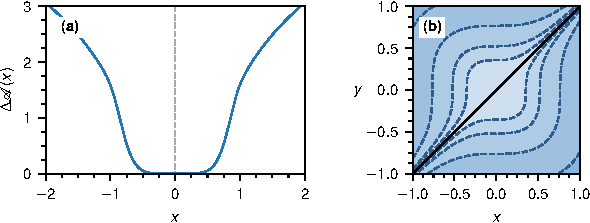
\includegraphics{fluctuations/line.pdf}
  \end{center}
  \caption{(a) Free energy $\Delta\mathscr{A}(x)$ of a particle under a potential $U(x,y) = \frac{1}{2}\kappa(x^{3}-y^{3})^{2}$. (b) Configuration space (black line) and energy level sets.}
  \label{fig:line}
\end{figure}

\subsubsection*{Cone-plane intersection}

Consider a particle constrained to move on the intersection curve between the right-circular cone defined by $x^{2} + y^{2} = z^{2}$ and the $yz$ plane (defined by $x = 0$).
Mathematically, the intersection curve is the zero level set of the following map:
%
\begin{equation}
  f: \mathbb{R}^{3} \to \mathbb{R}^{2},
  \quad\text{defined by}\quad
  f(x,y,z) =
  \begin{pmatrix}
    \abs{z} - \sqrt{x^{2} + y^{2}}\\
    x
  \end{pmatrix}
\end{equation}
%
As we can see from Fig.~\ref{fig:coneplane}, the configuration space $\Omega = f^{-1}(0)$ is nothing but the union of the lines $y = \pm z$, which intersect at the origin and create a singularity.
If we choose the $y$ coordinate as our \ac{cv} and compute the marginal density $\mathscr{P}(y)$ assuming a constraining potential $U(x, y, z) = \frac{1}{2}\kappa\Abs{f}^{2}$, we find (sans normalization)
%
\begin{equation}
  \mathscr{P}(y) = \int \dd{x}\,\dd{z}\,\exp\left\{-\tfrac{1}{2}\beta\kappa\left[\left(\smash[b]{\abs{z} - \sqrt{\smash[b]{x^{2} + y^{2}}}}\right)^{2} + x^{2}\right]\right\}.
\end{equation}
%
Although the above integral is unwieldy,%
\footnote{Or at least, I found it hard to integrate it exactly.}
we can find the following limiting cases after straightforward algebra
%
\begin{equation}
  \mathscr{P}(0) = \frac{3\pi}{\beta\kappa}
  \quad\text{and}\quad
  \mathscr{P}(y) \sim \left(\frac{2\pi}{\beta\kappa}\right)\left[1+\erf\left(\sqrt{\tfrac{1}{2}{\beta\kappa y^{2}}}\right)\right],
  \quad y \gg \sqrt{\smash[b]{\beta\kappa}},
\end{equation}
%
leading to a free-energy difference $\Delta\mathscr{A}(y) = \mathscr{A}(y) - \mathscr{A}(0)$ of the form
%
\begin{equation}
  \Delta\mathscr{A}(y) = -\beta^{-1} \log\left\{\left(\frac{2}{3}\right)\left[1+\erf\left(\sqrt{\tfrac{1}{2}{\beta\kappa y^{2}}}\right)\right]\right\},
  \quad y \gg \sqrt{\smash[b]{\beta\kappa}}.
\end{equation}
%
Clearly, in this case, the free energy is actually \emph{higher} for the singular value $y = 0$ of the \ac{cv}, leading to a free-energy barrier of $-\beta^{-1}\log(4/3)$ between points with $y < 0$ and $y > 0$.
This barrier can be explained by considering the energy level sets around $\Omega$.
%
\begin{figure}
  \begin{center}
    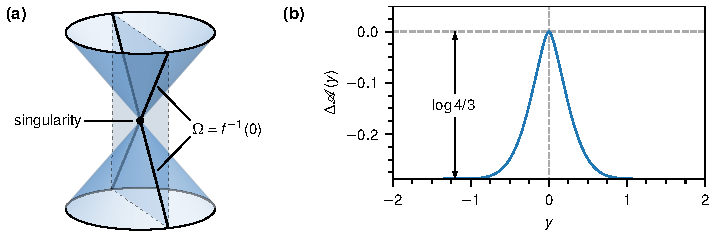
\includegraphics{fluctuations/coneplane.pdf}
  \end{center}
  \caption{Cone plane free}
  \label{fig:coneplane}
\end{figure}
